\subsection{Kontrolenhedens main}
Kontrolenhedens main har til ansvar at sende beskeder fra PC’en til Motorkontrolenheden og modsat.
For at kunne læse fra to forskellige steder på samme tid oprettes to tråde med hver sin trådfunktion \textit{fromMcToPc()} og \textit{fromPcToMc()}.
Trådenes funktionalitet illustreres på figur \ref{fig:controlunit_main}

\begin{figure} [H]
\centering
	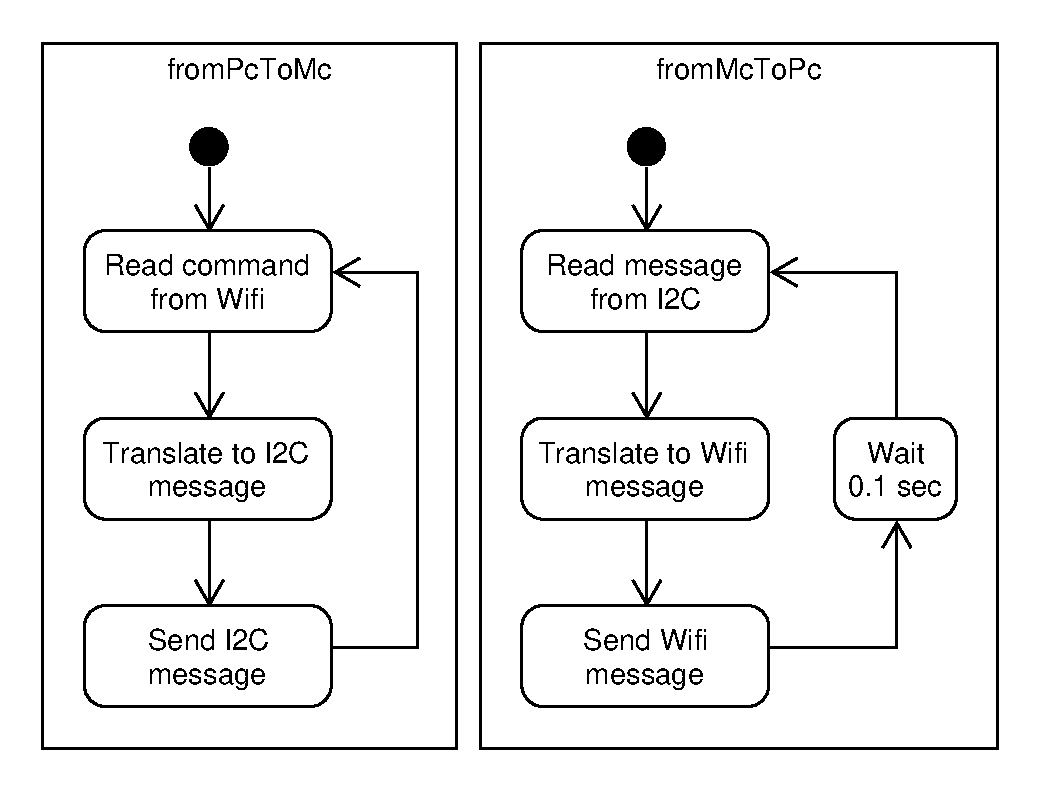
\includegraphics[width=0.8\textwidth]{controlunit_main.pdf}
	\captionof{figure}{Beskrivelse af Kontrolenhedens to tråde}
	\label{fig:controlunit_main}
\end{figure}

Før de to tråde sættes i gang oprettes der I2C-forbindelse til PSoC'en og Wifi-forbindelse til PC'en.\\
I main er der sat en default Wifi-port.
Hvis der ønskes at blive brugt en anden port, kan dette specificeres ved programstart. 
Hvis porten ikke er ledig, tælles den op indtil der findes en ledig port. 
På den måde undgås det at programmet ikke kan bruges.